\section{Beispiele}
\subsection{Pull-Up Treiber}
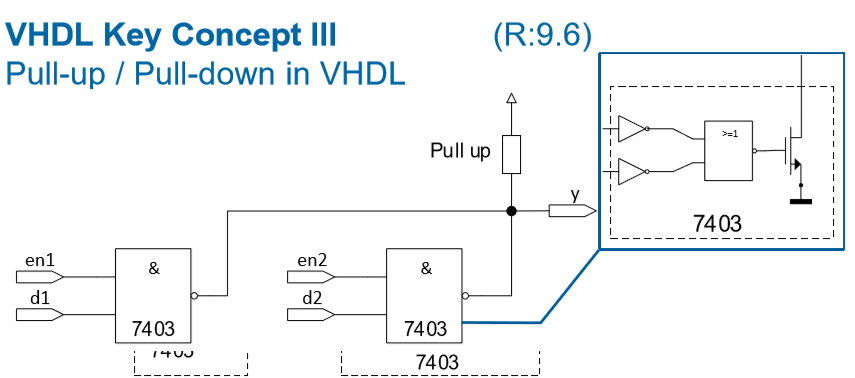
\includegraphics[width=\columnwidth]{Images/pullup}
\begin{lstlisting}
pull_up : y <= 'H';

p1 : process(en1, d1)
	begin
		y <= 'Z';
		if en1 = '1' and d1 = '1' then
			y <= '0';
		end if;
	end process;
	
p2 : process (en2, d2)
	begin
		y <= 'Z'
		if en2 = '1' and d2 = '1' then
			y <= '0';
		end if;
	end process;
\end{lstlisting}

\subsection{Bidirektionaler Bus}
\begin{center}
	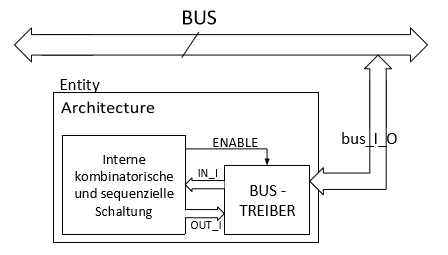
\includegraphics[width=0.8\columnwidth]{Images/bus}
\end{center}
\begin{lstlisting}
bus_write_p : process(enable, out_i)
	begin
		if enable = '1' then
			bus_i_o <= out_i;
		else
			bus_i_o <= (others => 'Z');
		end if;
	end process;
	
	bus_read : in_i <= bus_i_o; -- paralleler lesevorgang
\end{lstlisting}


\subsection{Latch}
\begin{center}
	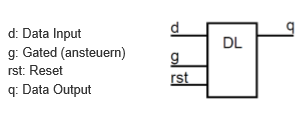
\includegraphics[width=0.5\columnwidth]{Images/latch}
\end{center}
Um ein Speicherverhalten zu simulieren, kann ein Latch verwendet werden. 
\begin{lstlisting}
process(rst, d, g)
begin
	if (rst = '1') then
		q <= '0' 
	elsif (g = '0') then
		q <= d
	else 
		null
end
\end{lstlisting}